
\begin{center}
    \begin{tikzpicture} [scale=0.8, transform shape]%show background rectangle,
        \tikzstyle{every node} = [draw, shape = rectangle, node distance=0mm, minimum width=5mm, minimum height=5.2mm]
        \node[draw=black, thick, label=below:Channel 2] (channel2) {
            \begin{tikzpicture}
                \node (puIdle) [fill=red!40, minimum width=30mm] {\small  Busy};%
            \end{tikzpicture}
        };
        \node[draw=black, thick, label=below:Channel 1] (channel1) [above=of channel2, yshift=7.5mm] {
            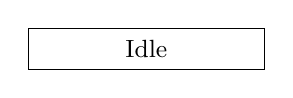
\begin{tikzpicture}
                \node (puBusy) [minimum width=30mm] {\small  Idle};
            \end{tikzpicture}
        };
        \node[draw=black, thick, label=below:Channel 3] (channel3) [below=of channel2, yshift=-7.5mm] {
            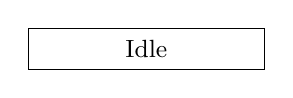
\begin{tikzpicture}
                \node (puBusy) [ minimum width=30mm] {\small  Idle};
            \end{tikzpicture}
        };
        \node[draw=black, thick, label=below:Channel 4] (channel4) [below=of channel3, yshift=-7.5mm] {
            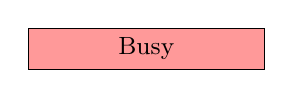
\begin{tikzpicture}
                \node (puBusy) [fill=red!40, minimum width=30mm] {\small  Busy};
            \end{tikzpicture}
        };

        \node[draw=white, thick] (pu1) [left=of channel1, xshift=-1mm] {
            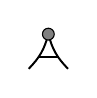
\begin{tikzpicture} [scale=0.5]
            \draw [line width=0.25mm, bend right = 15] (2, -0.44) to (2.5,0.44);
            \draw [line width=0.25mm, bend left = 15] (3, -0.44) to (2.5,0.44);
            \draw [line width=0.25mm] (2.25, -0.15) to (2.75,-0.15);
            %\draw [line width=0.25mm] (2.5, -0.44) to (2.5,0.44);
            \draw [fill=gray] (2.5,0.44) circle(1.5mm);

            \end{tikzpicture}
        };

        \node[draw=white, thick] (pu2) [left=of channel2, xshift=-1mm] {
            
\begin{tikzpicture} [scale=0.5]
            \draw [line width=0.25mm, bend right = 15, red] (2, -0.44) to (2.5,0.44);
            \draw [line width=0.25mm, bend left = 15, red] (3, -0.44) to (2.5,0.44);
            \draw [line width=0.25mm, red] (2.25, -0.15) to (2.75,-0.15);
            %\draw [line width=0.25mm] (2.5, -0.44) to (2.5,0.44);
            \draw [fill=red, red] (2.5,0.44) circle(1.5mm);

            \draw [line width=0.25mm, red] (2.5, 0.725) to (2.5,1.0);
            \draw [line width=0.25mm, red] (2.65, 0.65) to (2.825,0.85);
            \draw [line width=0.25mm, red] (2.725, 0.44) to (3,0.44);
            \draw [line width=0.25mm, red] (2.35, 0.65) to (2.175,0.85);
            \draw [line width=0.25mm, red] (2.275, 0.44) to (2,0.44);

            \end{tikzpicture}
        };

        \node[draw=white, thick] (pux1) [left=of pu2, xshift=-1mm] {
            
\begin{tikzpicture} [scale=0.5]
            \draw [line width=0.25mm, bend right = 15, red] (2, -0.44) to (2.5,0.44);
            \draw [line width=0.25mm, bend left = 15, red] (3, -0.44) to (2.5,0.44);
            \draw [line width=0.25mm, red] (2.15, -0.3) to (2.85,-0.3);
            \draw [line width=0.25mm, red] (2.25, -0.15) to (2.75,-0.15);
            \draw [line width=0.25mm, red] (2.35, 0) to (2.65,0);
            %\draw [line width=0.25mm] (2.5, -0.44) to (2.5,0.44);
            \draw [fill=red, red] (2.5,0.44) circle(1.5mm);

            \draw [line width=0.25mm, red] (2.5, 0.725) to (2.5,1.0);
            \draw [line width=0.25mm, red] (2.65, 0.65) to (2.825,0.85);
            \draw [line width=0.25mm, red] (2.725, 0.44) to (3,0.44);
            \draw [line width=0.25mm, red] (2.35, 0.65) to (2.175,0.85);
            \draw [line width=0.25mm, red] (2.275, 0.44) to (2,0.44);

            \end{tikzpicture}
        };

        \node[draw=white, thick] (pux2) [left=of pux1, xshift=-1mm] {
            
\begin{tikzpicture} [scale=0.5]
            \draw [line width=0.25mm, bend right = 15, red] (2, -0.44) to (2.5,0.44);
            \draw [line width=0.25mm, bend left = 15, red] (3, -0.44) to (2.5,0.44);
            \draw [line width=0.25mm, red] (2.15, -0.3) to (2.85,-0.3);
            \draw [line width=0.25mm, red] (2.25, -0.15) to (2.75,-0.15);
            \draw [line width=0.25mm, red] (2.35, 0) to (2.65,0);
            %\draw [line width=0.25mm] (2.5, -0.44) to (2.5,0.44);
            \draw [fill=red, red] (2.5,0.44) circle(1.5mm);

            \draw [line width=0.25mm, red] (2.5, 0.725) to (2.5,1.0);
            \draw [line width=0.25mm, red] (2.65, 0.65) to (2.825,0.85);
            \draw [line width=0.25mm, red] (2.725, 0.44) to (3,0.44);
            \draw [line width=0.25mm, red] (2.35, 0.65) to (2.175,0.85);
            \draw [line width=0.25mm, red] (2.275, 0.44) to (2,0.44);

            \end{tikzpicture}
        };

        \node[draw=white, thick] (pu3) [left=of channel3, xshift=-1mm] {
            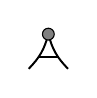
\begin{tikzpicture} [scale=0.5]
            \draw [line width=0.25mm, bend right = 15] (2, -0.44) to (2.5,0.44);
            \draw [line width=0.25mm, bend left = 15] (3, -0.44) to (2.5,0.44);
            \draw [line width=0.25mm] (2.25, -0.15) to (2.75,-0.15);
            %\draw [line width=0.25mm] (2.5, -0.44) to (2.5,0.44);
            \draw [fill=gray] (2.5,0.44) circle(1.5mm);

            \end{tikzpicture}
        };

        \node[draw=white, thick] (pu4) [left=of channel4, xshift=-1mm] {
            
\begin{tikzpicture} [scale=0.5]
            \draw [line width=0.25mm, bend right = 15, red] (2, -0.44) to (2.5,0.44);
            \draw [line width=0.25mm, bend left = 15, red] (3, -0.44) to (2.5,0.44);
            \draw [line width=0.25mm, red] (2.25, -0.15) to (2.75,-0.15);
            %\draw [line width=0.25mm] (2.5, -0.44) to (2.5,0.44);
            \draw [fill=red, red] (2.5,0.44) circle(1.5mm);

            \draw [line width=0.25mm, red] (2.5, 0.725) to (2.5,1.0);
            \draw [line width=0.25mm, red] (2.65, 0.65) to (2.825,0.85);
            \draw [line width=0.25mm, red] (2.725, 0.44) to (3,0.44);
            \draw [line width=0.25mm, red] (2.35, 0.65) to (2.175,0.85);
            \draw [line width=0.25mm, red] (2.275, 0.44) to (2,0.44);

            \end{tikzpicture}
        };
    \end{tikzpicture}
    \begin{tikzpicture}
    

        \iffalse
        \node[draw=white, thick, label=left:\tiny Primary User] (pu) [left=of pu3, xshift=-1cm] {
            \begin{tikzpicture} [scale=0.5]
            \draw [line width=0.25mm, bend right = 15] (2, -0.44) to (2.5,0.44);
            \draw [line width=0.25mm, bend left = 15] (3, -0.44) to (2.5,0.44);
            \draw [line width=0.25mm] (2.25, -0.15) to (2.75,-0.15);
            %\draw [line width=0.25mm] (2.5, -0.44) to (2.5,0.44);
            \draw [fill=gray] (2.5,0.44) circle(1.5mm);

            \end{tikzpicture}
        };

        \node[draw=white, thick] (su) [right=of su2, xshift=1cm, yshift=-1mm] {
            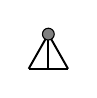
\begin{tikzpicture} [scale=0.5]
            \draw [line width=0.25mm] (2, -0.44) to (2.5,0.44);
            \draw [line width=0.25mm] (3, -0.44) to (2.5,0.44);
            \draw [line width=0.25mm] (2, -0.44) to (3,-0.44);
            \draw [line width=0.25mm] (2.5, -0.44) to (2.5,0.44);
            \draw [fill=gray] (2.5,0.44) circle(1.5mm);

            \end{tikzpicture}
        };
        \fi
    \end{tikzpicture}
\begin{center}
%\only<1>{In CRNs there are some Primary users and some Secondary users, some of the Primary users remain mostly Idle, where a Secondary user can operate.}
%\only<2>{If the Idleness of a Primary user change, the Secondary user's operation can get interrupted.}
%\only<3>{The secondary user need to switch to a new Idle channel.}
%\only<4>{Now. the question is what do we focus in such CRNs?}
\end{center}
\iffalse
\only<5>{
\begin{textblock*}{0.6\textwidth}(0.28\textwidth,0.4\textheight)
\textblockcolour{green!25!white}
\centering
\vspace{5mm}
  \textcolor{red}{Motivation}\\
  significant spectrum under-utilization in traditional spectrum management~\cite{akyildiz2006next}
\vspace{5mm}
\end{textblock*}
}
\fi
\end{center}
